\chapter{Creación del sistema}

El sistema que vamos a crear constará de las siguientes partes. Primero sobre las máquinas con SO Windows se instalará una máquina virtual Ubuntu sobre Virtualbox para trabajar en un entorno linux. A día de hoy existen formas de trabajar directamente con Docker en sistemas Windows tanto por CLI (Command Line Interface) como a través de una interfaz gráfica, aunque éstas se basan en emular el kernel de linux. Para este caso se ha optado por trabajar en un entorno linux conocido para hacer más simple el despligue del sistema.

Dentro de dicha máquina Ubuntu se instalará el propio Docker. Mediante Docker crearemos diferentes contenedores. Cada uno de esos contenedores se crearán a partir de una imagen de Ubuntu que vendrá con ROS instalado. Esa imagen sera la que aparece en el Docker Hub como \emph{osrf/ros:indigo-desktop}. Estas máquinas se comunicarán entre ellas mediante una red creada con la herramienta \emph{network} de Docker.

El esquema del sistema vendría a ser el que se muestra en la Figura \ref{fig:esquemaOriginal}.
\begin{figure}[H] % Con el parámetro H la imagens se muestra justo en el sitio en el que se ha definido
	\centering
	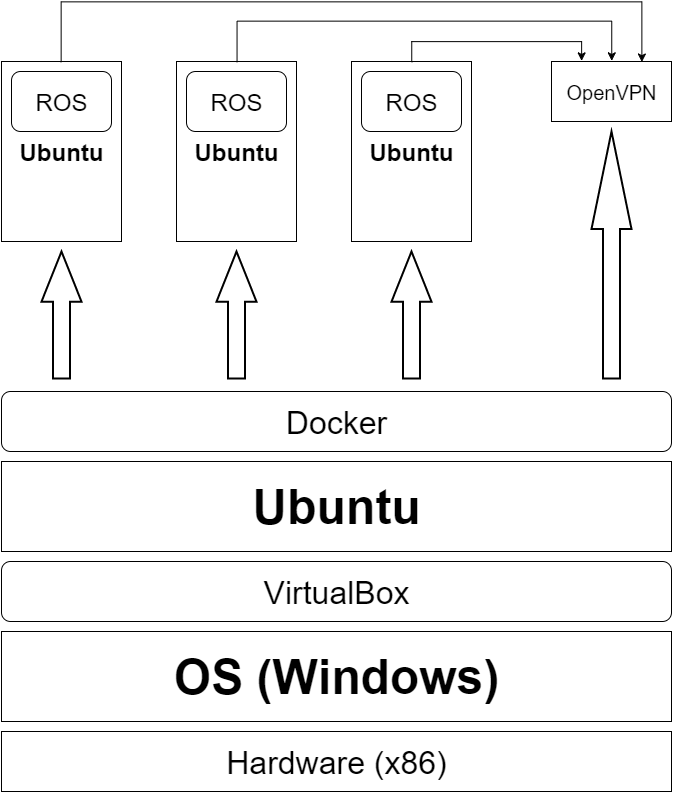
\includegraphics[width=0.8\textwidth]{esquemaOriginal}
	%		\includesvg{figuras/esquemaOriginal}
	\caption{Esquema del sistema en un ordenador x86}
	\label{fig:esquemaOriginal}
\end{figure}

Posteriormente integraremos nuestro sistema en una Raspberry Pi. El esquema del sistema aplicado en una Raspberry Pi se muestra en la Figura \ref{fig:esquemaRPi}.
\begin{figure}[H]
	\centering
	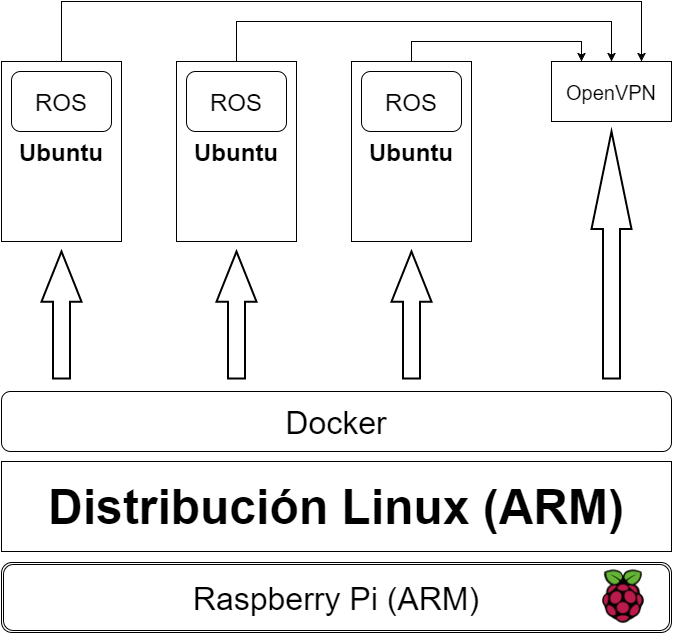
\includegraphics[width=0.8\textwidth]{esquemaRPi}
	%		\includesvg{figuras/esquemaRPi}
	\caption{Esquema del sistema en una Raspberry Pi}
	\label{fig:esquemaRPi}
\end{figure}

	\section{Crear el sistema con Docker}
	Lo primero que haremos será crear una serie de contenedores de docker con ROS dentro.
	
	\begin{enumerate}
		\item Creamos en tres terminales diferentes tres contenedores ROS.
		\begin{lstlisting}[style=consola,numbers=left]
$ docker run --name ros0 -it osrf/ros:indigo-desktop
$ docker run --name ros1 -it osrf/ros:indigo-desktop
$ docker run --name ros2 -it osrf/ros:indigo-desktop
		\end{lstlisting}
		
		\item Desde el host, creamos la red y conectamos los tres contenedores a ella.
		\begin{lstlisting}[style=consola,numbers=left]
$ docker network create red
a9ccfbd91df31be74881c7a7e65fbb0fdd6fec286debec6c72b1f627bb0e2ad0
$ docker network ls
NETWORK ID          NAME                DRIVER
a9ccfbd91df3        red                 bridge              
6fb4fab5cc04        bridge              bridge              
a55fc7d11d74        none                null                
2c96fadb05a4        host                host                
$ docker network connect red ros0
$ docker network connect red ros1
$ docker network connect red ros2
		\end{lstlisting}
		
		\item Probamos el ejemplo anterior con nodos ROS pero esta vez dentro de los contenedores Docker. Simplemente hay que tener en cuenta que hay que configurar la variable \emph{ROS\_MASTER\_URI} para que apunte a \emph{ros0}, que es la dirección del contenedor que ejecutará \emph{roscore}.
		
		\begin{enumerate}
			\item Lanzamos \emph{roscore} en \emph{ros0}.
			\begin{lstlisting}[style=consola]
root@d55b47478e2c:/# roscore
			\end{lstlisting}
			
			\item En \emph{ros1} y \emph{ros2} configuramos la variable que indica donde se está ejecutando \emph{roscore}
			\begin{lstlisting}[style=consola]
$ ROS_MASTER_URI=http://ros0:11311/
			\end{lstlisting}
			
			\item Tanto para \emph{ros1} como para \emph{ros2}, hace falta poner en la variable \emph{ROS\_IP} la IP del conentedor. Esto sirve para que el \emph{roscore} pueda encontrar los nodos. Lo haremos mirando dentro de cada contenedor la IP \textbf{correspondiente a la red creada por nosotros}. En nuestro caso se haría de la siguiente manera.
			\begin{lstlisting}[style=consola]
root@9d1dbcbf599c:~/catkin_ws# export ROS_IP=172.18.0.4
root@ee37147629e4:~/catkin_ws# export ROS_IP=172.18.0.3
			\end{lstlisting}
			
			\item Con todo el ejemplo creado y compilado dentro de \emph{ros1} y \emph{ros2}, lanzamos en \emph{ros1} el listener.
			\begin{lstlisting}[style=consola]
root@ee37147629e4:~/# rosrun prueba listener	
			\end{lstlisting}
			
			\item Y probamos a escribir mediante el talker.
			\begin{lstlisting}[style=consola]
root@9d1dbcbf599c:~/# rostopic pub -1 /chatter std_msgs/String PruebaMensaje
			\end{lstlisting}
			\begin{lstlisting}[style=consola]
root@9d1dbcbf599c:~/# rosrun prueba listener
[ INFO] [1447688515.499505438]: I heard: [PruebaMensaje]
			\end{lstlisting}

		\end{enumerate}
		
	\end{enumerate}
	
	\section{Aplicaciones para el sistema}
	Una vez creado el sistema solo faltaria programarlo para que haga lo que nosotros queramos. En el mundo de la robótica existen una gran cantidad de utilidades para implementar, desde movimientos de piezas o de partes, recogida de información de sensores,...
	
	Como no se pretende en este documento crear aplicaciones robóticas concretas, nos vamos a limitar a mostrar un ejemplo de aplicación para nuestro sistema. En este caso se ha optado por obtener imágenes de una Webcam, un ejemplo sencillo a la par que útil.
		
		\subsection{Obtener imágenes de una Webcam}
		Lo primero que hay que tener en cuenta es que para que nuestra máquina virtual detecte la Webcam es necesario instalar el \textit{Oracle VM VirtualBox Extension Pack}. Es una extensión de VirtualBox que permite que las máquinas virtuales interactúen con dispositivos USB 2.0 y 3.0, controladores Bluetooth o Webcams integradas, entre otros.
		
		Una vez instalado hay que habilitar la Webcam desde las opciones de VirtualBox. Para ello la seleccionamos en el menú Webcam de la sección Devices de nuestra máquina virtual, ta y como aparece en la Figura \ref{fig:VBoxWebcam}.
		\begin{figure}[H]
			\centering
			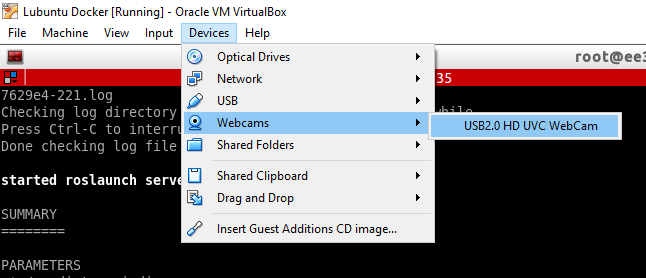
\includegraphics{VBoxWebcam}
			\caption{Activación de la Webcam en VirtualBox}
			\label{fig:VBoxWebcam}
		\end{figure}
		
		Para obtener imágenes de una Webcam haremos lo siguiente.
		\begin{enumerate}
			\item Lanzamos \emph{roscore} en \emph{ros0}.
			\begin{lstlisting}[style=consola]
root@d55b47478e2c:/# roscore
			\end{lstlisting}
			
			\item En \emph{ros1} y \emph{ros2} configuramos la variable que indica donde se está ejecutando \emph{roscore}
			\begin{lstlisting}[style=consola]
$ ROS_MASTER_URI=http://ros0:11311/
			\end{lstlisting}
			
			\item En cualquiera de los otros nodos, por ejemplo en \emph{ros1}, añadiremos el paquete \textit{usb\_cam} de ROS a workspace de catkin de ese contenedor de la siguiente manera:
			\begin{lstlisting}[style=consola,numbers=left]
root@ee37147629e4:~/catkin_ws# cd src
root@ee37147629e4:~/catkin_ws/src# git clone "https://github.com/bosch-ros-pkg/usb_cam.git"
root@ee37147629e4:~/catkin_ws/src# cd ..
root@ee37147629e4:~/catkin_ws# catkin_make
#
# Se omite la salida de la compilacion por ser demasiado larga
#
			\end{lstlisting}
			
			\item Lanzamos el ejemplo que nos incluye el paquete para probar su funcionamiento.
			\begin{lstlisting}[style=consola,numbers=left]
root@ee37147629e4:~/catkin_ws/# cd src/usb_cam/launch
root@ee37147629e4:~/catkin_ws/src/usb_cam/launch# roslaunch usb_cam-test.launch
... logging to /root/.ros/log/55cdb074-bce6-11e5-9018-0242ac110002/roslaunch-ee37147629e4-221.log
Checking log directory for disk usage. This may take awhile.
Press Ctrl-C to interrupt
Done checking log file disk usage. Usage is <1GB.

started roslaunch server http://ee37147629e4:39700/

SUMMARY
========

PARAMETERS
* /rosdistro: indigo
* /rosversion: 1.11.13
* /usb_cam/camera_frame_id: usb_cam
* /usb_cam/image_height: 480
* /usb_cam/image_width: 640
* /usb_cam/io_method: mmap
* /usb_cam/pixel_format: mjpeg
* /usb_cam/video_device: /dev/video0

NODES
/
image_view (image_view/image_view)
usb_cam (usb_cam/usb_cam_node)

ROS_MASTER_URI=http://ros0:11311/

core service [/rosout] found
			\end{lstlisting}
			
			\item Si todo ha ido bien, debería aparece una ventana como la que aparece en la Figura \ref{fig:VBoxWebcam2}, en la que aparecerá la imágen de la Webcam.
			\begin{figure}[H]
				\centering
				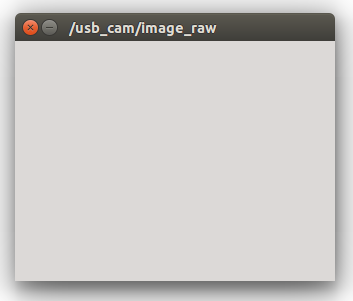
\includegraphics{VBoxWebcam2}
				\caption{Ventana con la imagen de la Webcam}
				\label{fig:VBoxWebcam2}
			\end{figure}
			
		\end{enumerate}
		
		\subsection{Otras aplicaciones}
		A parte de la captura de imágenes de una Webcam, podemos elaborar una serie de aplicaciones con ROS, basandonos o no en librerías existentes, que se basen en áreas como por ejemplo \cite{ros-wikipedia}:
		\begin{itemize}
			\item Percepción
			\item Identificación de Objetos
			\item Segmentación y reconocimiento
			\item Reconocimiento facial
			\item Reconocimiento de gestos
			\item Seguimiento de objetos
			\item Egomoción
			\item Comprensión de movimiento
			\item Estructura de movimientos (SFM)
			\item Visión estéreo: percepción de profundidad mediante el uso de dos cámaras
			\item Movimientos
			\item Robots móviles
			\item Control
			\item Planificación
			\item Agarre de objetos
		\end{itemize}